\documentclass[tikz]{standalone}

\usepackage{amsmath}
\usepackage{unicode-math}
\usepackage{mathtools}
\usepackage{derivative}

\setmainfont{Stix Two Text}
\setmathfont{Stix Two Math}

\usetikzlibrary{arrows.meta,fit,positioning}

\renewcommand{\familydefault}{\sfdefault}

% prefix equation numbers with section number
\numberwithin{equation}{section}

\DeclarePairedDelimiter{\ceil}{\lceil}{\rceil}
\DeclarePairedDelimiter{\floor}{\lfloor}{\rfloor}
\DeclarePairedDelimiter{\abs}{\lvert}{\rvert}
\DeclarePairedDelimiter{\norm}{\lVert}{\rVert}
\DeclarePairedDelimiter{\bra}{\langle}{\rvert}
\DeclarePairedDelimiter{\ket}{\lvert}{\rangle}
\DeclarePairedDelimiter{\expval}{\langle}{\rangle}
\DeclarePairedDelimiter{\norder}{\mathcolon}{\mathcolon}
\DeclarePairedDelimiter{\anorder}{\typecolon}{\typecolon}
	
\newcommand{\laplace}{\mbfnabla^2}
\newcommand{\trans}{{\scriptscriptstyle\mathsf{T}}}

\newcommand{\vdot}{\cdot}
\newcommand{\vcross}{\vectimes}
\newcommand{\vb}[1]{\symbfup{#1}}
\newcommand{\vu}[1]{\hat{\vb{#1}}}
\newcommand*\dd[2][\relax]{\mathop{\ifx\relax#1\odif{#2}\else \odif[order={#1}]{#2}\fi\,}}

\newcommand{\vacuum}{\ket*{\vb{0}}}

\DeclareMathOperator{\trace}{Tr}
\DeclareMathOperator{\sinc}{sinc}

\AtBeginDocument{
	\let\Re\relax
	\let\Im\relax
	\DeclareMathOperator{\Re}{Re}
	\DeclareMathOperator{\Im}{Im}

	\renewcommand{\div}{\mathop{\mbfnabla\vdot}}
	\newcommand{\curl}{\mathop{\mbfnabla\vectimes}}
}

\DeclarePairedDelimiterX{\comm}[2]{[}{]}{#1,#2}

\DeclarePairedDelimiterX{\braket}[2]{\langle}{\rangle}{#1\delimsize\vert#2}
\DeclarePairedDelimiterX{\ketbra}[1]{\lvert}{\rvert}{#1\rangle\delimsize\langle#1}



\usetikzlibrary{decorations.pathmorphing}

\begin{document}
	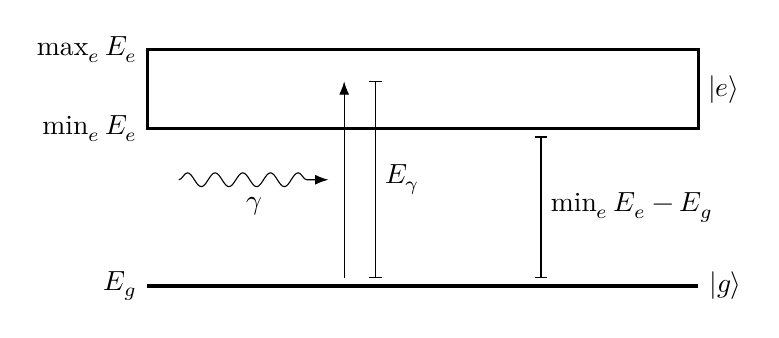
\begin{tikzpicture}[
		photon/.style={-Latex, decorate, decoration={snake, post length=1mm}},
	]
		\draw[very thick] (0,0) -- ++(7,0) node[right] {$\ket{g}$};
		\draw (0,2) node[left] {$\min_eE_e$} ++(0,1) node[left] {$\max_eE_e$};
		
		\draw[very thick] node[left] {$E_g$} (0,2) rectangle ++(7,1);
		\draw (7,2.5) node[right] {$\ket{e}$};
		
		\draw[-Latex] (2.5,0.1) -- ++(0,2.5);
		\draw[photon] (0.4,1.35) -- ++(1.9,0) node[midway, below, yshift=-0.1cm] {$\gamma$};
		
		\draw[Bar-Bar] (5,0.1) -- ++(0,1.8) node[midway, right] {$\min_eE_e-E_g$};
		\draw[Bar-Bar] (2.9,0.1) -- ++(0,2.5) node[midway, right] {$E_\gamma$};
	\end{tikzpicture}
\end{document}
